% !TEX root =  ../ms.tex
\section{Introduction}
\label{sec : introduction}
According to the inclusion criteria of the study, a total of 239 kidney transplant patients were included in the data set. The transplantation characteristics of these patients is presented in Table \ref{tab : baseline_characteristics}. The data set also includes periodical measurements of serum creatinine (SCr) and protein creatinine ratio (PCR), which are biomarkers used to check the state of the transplant. The median number of repeated SCr and PCR measurements per patient are 45 and 37, respectively. For SCr 95\% of the observations are taken before 6 years, while for PCR they are taken before 5.4 years. The median time between two SCr measurements is 10 days, while the same for PCR is 14 days.

\begin{table}[!htb]
\begin{center}
\caption{Observed transplantation characteristics of the studied population (n = 239).}
\label{tab : baseline_characteristics}
\begin{tabular}{llr}
\Hline
\multicolumn{3}{c}{Quantitative characteristics} \\
\hline
Name & Abbreviation & Mean (SD) \\ 
\hline
Receiver age (at baseline) & rec\_age & 50.70 (13.09) \\
Donor age & d\_age & 49.73 (12.66) \\
Donor BMI & d\_bmi & 25.10 (4.43) \\
Receiver BMI & rec\_bmi & 25.43 (4.31) \\
Cold ischemia time (minutes) & cit & 887.25 (522.95)\\
\#HLA A, B and DR mismatches & hla & 2.81 (1.57)\\
Panel reactive antibody (\%) & pra & 4.81 (14.20) \\
\#Days on dialysis before transplant & dial\_days & 1334.91 (1283.93)\\
\#Anti-hypertensive medicaments & ah\_nr & 1.58 (0.96)\\
\hline
\\
\multicolumn{3}{c}{Categorical characteristics}\\
\hline
Name & Abbreviation & Category (\%) \\
\hline
Receiver gender & rec\_gender & Female (42.68 \%)\\
Donor gender & d\_gender & Female (56.49 \%)\\
Delayed graft function after transplant & dgf & No (67.78 \%)\\
Previous transplantation & prev\_tp & No (84.45 \%)\\
Diabetes mellitus & dm & No (84.52 \%)\\
Known cardiovascular events before transplant & hvdis & No (61.92 \%)\\
Deceased donor & d\_cadaveric & No (25.94 \%)\\
\hline     
\end{tabular}
\end{center}
\end{table}

In the cohort, 44 out of 239 patients observed graft failure (death-censored). The survival probability one year post transplantation is 97.87\%. The graft survival probabilities and 95\% CI estimated using Kaplan-Meier estimator are presented in Figure \ref{fig : km_curve}. 

\begin{figure}[!htb]
\centerline{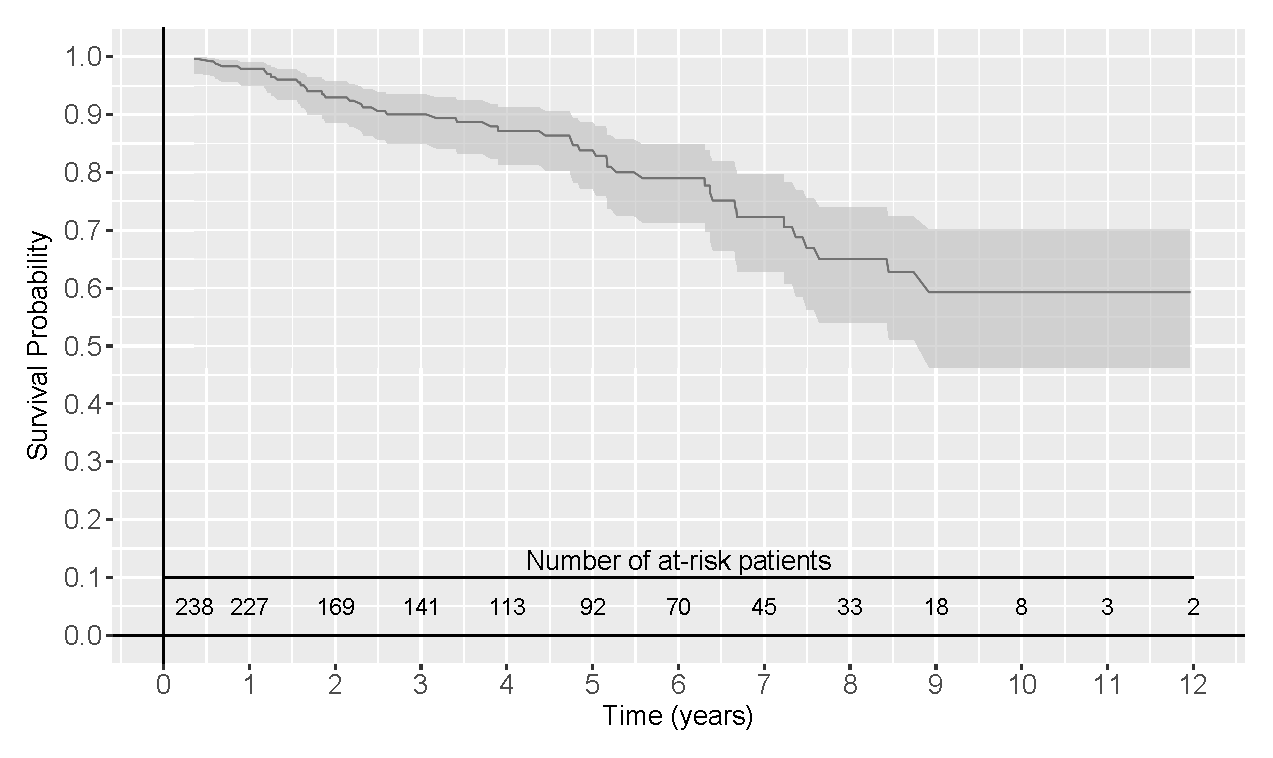
\includegraphics[width=\columnwidth]{images/km.eps}}
\caption{Graft survival probabilities and 95\% CI estimated using Kaplan-Meier estimator.}
\label{fig : km_curve}
\end{figure}
